\documentclass{aa}
\usepackage{graphicx,txfonts}
\usepackage[hidelinks]{hyperref}
\journalname{Euclid Deep Field North}
\makeatletter
\renewcommand*\aa@manuscriptname{\quad\textnormal{Research report}}
\renewcommand*\aa@textidlineempty{\textit{Euclid Deep Field North}}
\AtBeginDocument{%
  \renewcommand*\aa@numarticle{}%
  \renewcommand*\aa@pageof{Page \thepage}%
}
\makeatother
\hypersetup{pdfauthor={Biswajit Jana}}
% The A&A class enables review line numbering at the end of the document.
% These are reader-facing research reports.
\renewcommand{\linenumbers}{\nolinenumbers}

\graphicspath{{../2026-11-15-day02/analysis/}}
\begin{document}
\hypersetup{pdftitle={Aperture-size sensitivity and five spectral case studies in Euclid Deep Field North}}
\title{Aperture-size sensitivity and five spectral case studies in Euclid Deep Field North}
\subtitle{Day 2. An eight-tile DR1-Foundation analysis}
\author{Biswajit Jana}
\institute{Independent researcher, United Kingdom}
\date{15 November 2026}
\abstract
{Catalogue apertures and slitless line measurements respond to source blending, spectral masks, and spatially varying observing conditions.}
{We test whether an exploratory H$\alpha$--aperture association persists when the size estimator, line measurement, and resampling unit change.}
{We match a $0.28^{\circ}$ field to eight MER catalogues and compare catalogue and direct VIS aperture measurements. Five sources are examined using NISP spectra, individual red-grism extractions where available, and external imaging or redshifts.}
{All 1576 selected objects have a morphology match, and 782 pass the imaging cuts. The catalogue Kron contrast is $+0.05166$ dex. For 398 common sources measured directly in VIS, adopting reliable red-grism H$\alpha$ flux gives $+0.01402$ dex, with whole-tile bootstrap endpoints $-0.0173$ and $+0.0443$ dex. One H$\alpha$-region signal repeats in 12 usable individual red extractions. A second combined-spectrum fit falls from formal S/N 21.23 to 1.14 after removal of one flagged bin.}
{The spatial comparison leaves the size association unresolved. Exposure-level repeatability and external spectroscopy constrain the interpretation of individual lines.}
\keywords{galaxies: photometry -- galaxies: statistics -- methods: data analysis -- techniques: spectroscopic}
\maketitle
\section{Introduction and sample}
Day 1 supplied original morphology for one contributing tile. The present pilot restores morphology coverage for eight tiles in a $0.28^{\circ}$ cone centred at ICRS RA $269.733^{\circ}$ and Dec $+66.018^{\circ}$ \citep{aussel2026}. Positive rank-0 H$\alpha$ fits at S/N~$\geq5$, catalogue redshift 0.90--1.50, redshift probability $\geq0.99$, and positive VIS aperture flux give 1576 exact matches. The original imaging cuts leave 782. Both grism spectra are available for 858 objects in three checked HATS partitions. The five case studies illustrate distinct measurement outcomes.

\section{Methods}
Kron contrasts use the high-minus-low H$\alpha$ difference in median log-radius within redshift and VIS-flux strata, weighted by object count. Direct VIS radii enclose half the signed, background-subtracted flux within $1.5''$. The local sky is estimated at $2.5''$--$3.5''$. The spatial check uses cells within tiles, with at least five objects per H$\alpha$ half, and resamples whole tiles in 4000 draws. The matched comparison uses the same objects under two H$\alpha$ estimators. Reliable red fits are identified by SPE Gaussian-fit code 212.

The NISP diagnostic fits a local linear continuum and a Gaussian of width $\sigma=30$~\AA{} at the SPE-predicted wavelength. It tests mask 0 and, separately, a rule admitting pixels that carry only the low-S/N warning. Adjusted S/N divides formal S/N by the larger of one and the sideband residual RMS in noise units. H$\alpha$-region fits can contain [N\,II] \citep{fumana2026,gabarra2026}.

\begin{table}[t]
\caption{H$\alpha$ contrasts in median log aperture radius.}
\label{tab:contrast}
\centering\small
\begin{tabular}{lrrr}
\hline\hline
Estimator & $N$ & $\Delta$ (dex) & Bootstrap endpoints\\
\hline
Kron, median H$\alpha$ &782&$+0.05166$&$+0.0204$, $+0.0761$\\
VIS, median H$\alpha$ &398&$+0.03363$&$-0.0116$, $+0.0710$\\
VIS, reliable red &398&$+0.01402$&$-0.0173$, $+0.0443$\\
VIS, reliable red &233&$+0.01719$&$-0.0211$, $+0.0624$\\
\hline
\end{tabular}
\tablefoot{Kron resamples objects. VIS resamples tiles. The first two VIS rows use $2.0''$ isolation. The last uses $2.5''$.}
\end{table}

\section{Results and discussion}
For the same 398 objects, changing the H$\alpha$ estimator lowers the VIS contrast by 0.01961 dex (Table~\ref{tab:contrast}). Three of the five eligible tiles give positive contrasts and two give negative contrasts. In linear units the reliable-red estimate and descriptive endpoints are $+3.3\%$ ($-3.9\%$, $+10.7\%$). Adjacent tiles can share systematics. The line-selected sample and the PSF-convolved aperture measurements limit intrinsic size inference.

\begin{figure*}[!t]
\centering
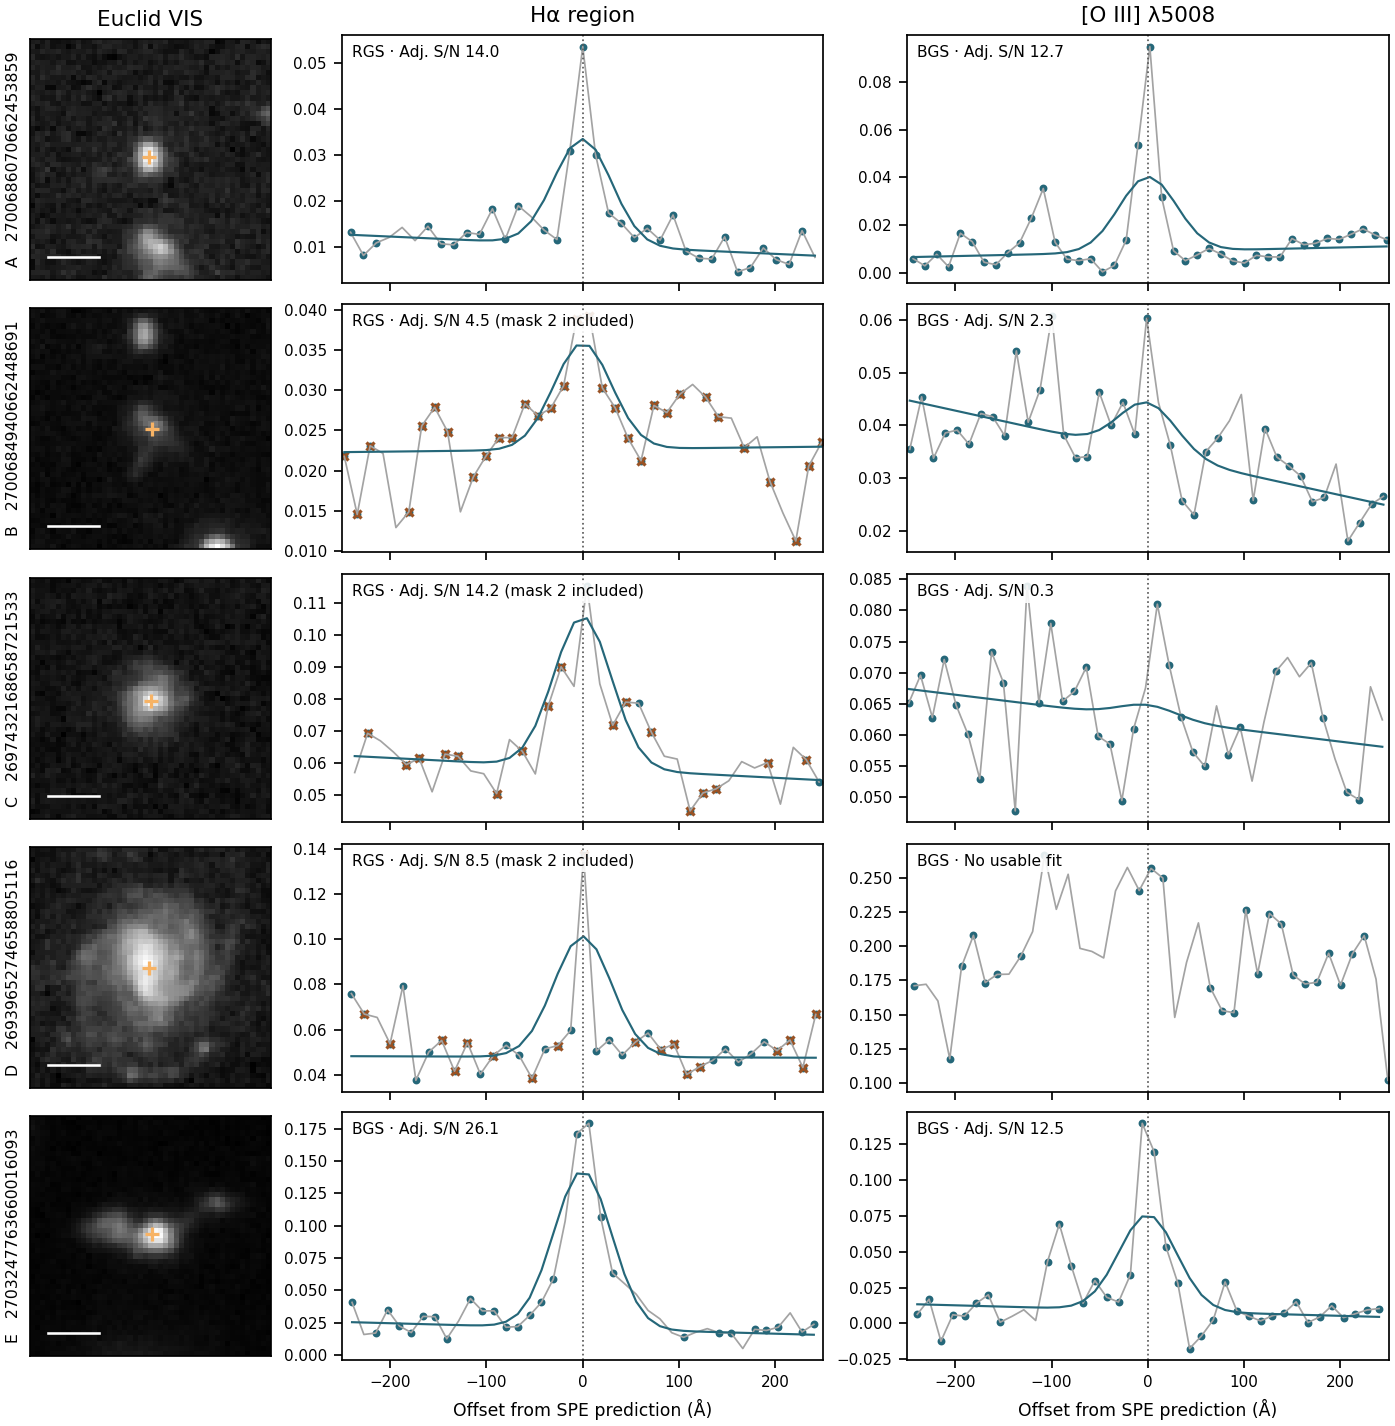
\includegraphics[width=.48\textwidth]{targets/five_source_diagnostics.png}
\caption{VIS stamps and H$\alpha$-region and [O\,III] $\lambda5008$ windows for the five DR1 sources. Dotted lines mark SPE-predicted wavelengths. Crosses identify bins admitted in the mask-2 sensitivity fit. The white image scale bars are $1''$.}
\label{fig:cases}
\end{figure*}

Sources A and B (Fig.~\ref{fig:cases}) are separated by $1.868''$. Their Q1 matches lie within $0.008''$ and $0.019''$. Independent Subaru HSC $i2$ detects both and leaves the shape of B's extension uncertain (Fig.~\ref{fig:pair}). A has strict adjusted S/N 14.02 and 12.69 for the H$\alpha$ region and [O\,III], respectively. All six bins in B's H$\alpha$ core carry the low-S/N warning. Its relaxed adjusted S/N is 4.50, and strict [O\,III] has S/N 2.28.

C has positive flux in all 12 usable red extractions, with formal S/N up to 7.98 and 6.93 in different directions without a listed contaminant in those fits. D's warning-inclusive formal S/N falls from 21.23 to 1.14 on removing one flagged bin. Its highest strict individual S/N is 2.34. E has strict adjusted blue-grism H$\alpha$ and [O\,III] S/N of 26.11 and 12.46. DESI gives $z=0.975547$ at $0.102''$ from E, compared with Euclid $z=0.975754$ \citep{desi2025}. Across 97 unique matches at $0.2''$, 81 agree to $|\Delta z|/(1+z_{\mathrm{DESI}})\leq0.002$. The fraction applies to the cross-matched subset.

\begin{figure}[!htbp]
\centering
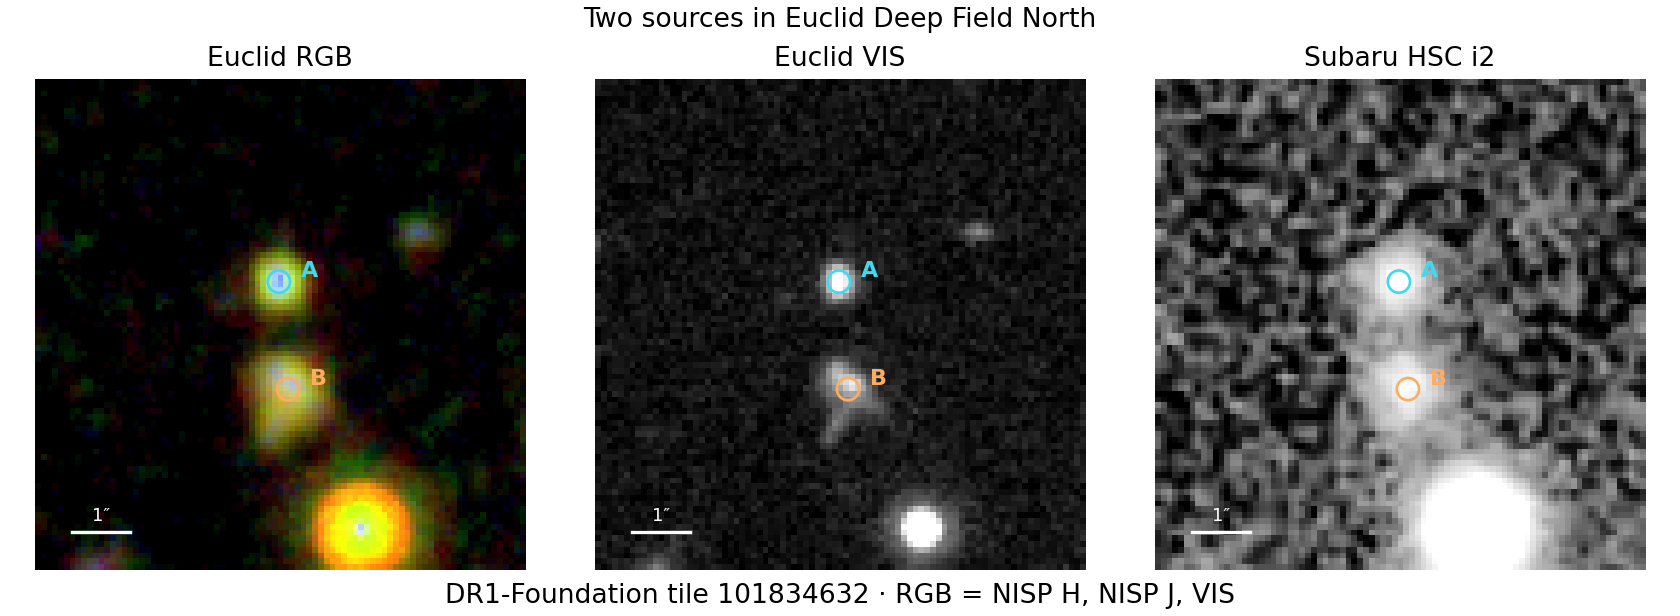
\includegraphics[width=\columnwidth]{targets/pair/Euclid_pair_RGB.png}
\caption{Observed close pair A and B. Left to right, Euclid VIS plus NISP J/H colour composite, Euclid VIS, and Subaru HSC $i2$. The circles mark sources $1.868''$ apart. Subaru shows both sources and leaves the shape of B's faint extension unresolved.}
\label{fig:pair}
\end{figure}

\section{Conclusions}
The direct VIS comparison remains inconclusive. The spectral cases identify a repeatable feature, a flagged-bin failure and a redshift with external support. B's origin and physical association with A remain unresolved.

\section*{Data availability}
The \href{https://github.com/Biswajit1999/daily-astro-notebooks/tree/master/euclid-dr1-foundation/2026-11-15-day02}{repository} provides analysis code, FITS stamps and source-level measurements. IRSA combined spectra DOI \href{https://doi.org/10.26131/IRSA680}{10.26131/IRSA680}.
\begin{acknowledgements}
This work has made use of the Data Release (DR1) data from the Euclid mission of the European Space Agency (ESA). NASA/IPAC IRSA distributes Euclid and the Subaru WISHES mosaic. DESI data were accessed through NOIRLab Astro Data Lab.
\end{acknowledgements}
\bibliographystyle{aa}
\bibliography{references}
\end{document}
